\chapter{League of Legends statistics}\label{app:lol_stats}
\begin{figure}[H]
	\centering
  \subfloat[Overview numerical]{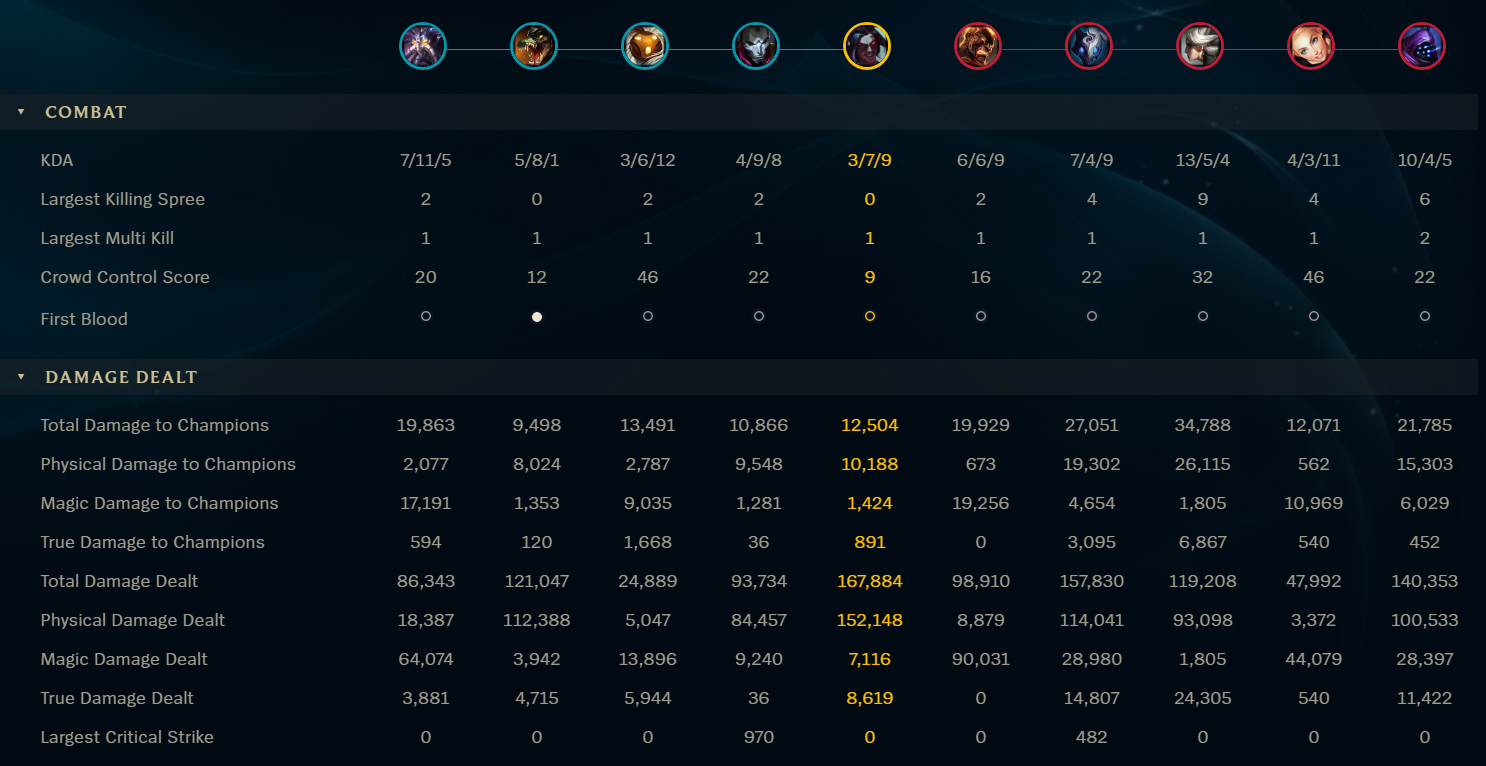
\includegraphics[width=\columnwidth, height=6cm]{source/images/lol_stats_1} }
	\qquad
	\subfloat[Overview graph]{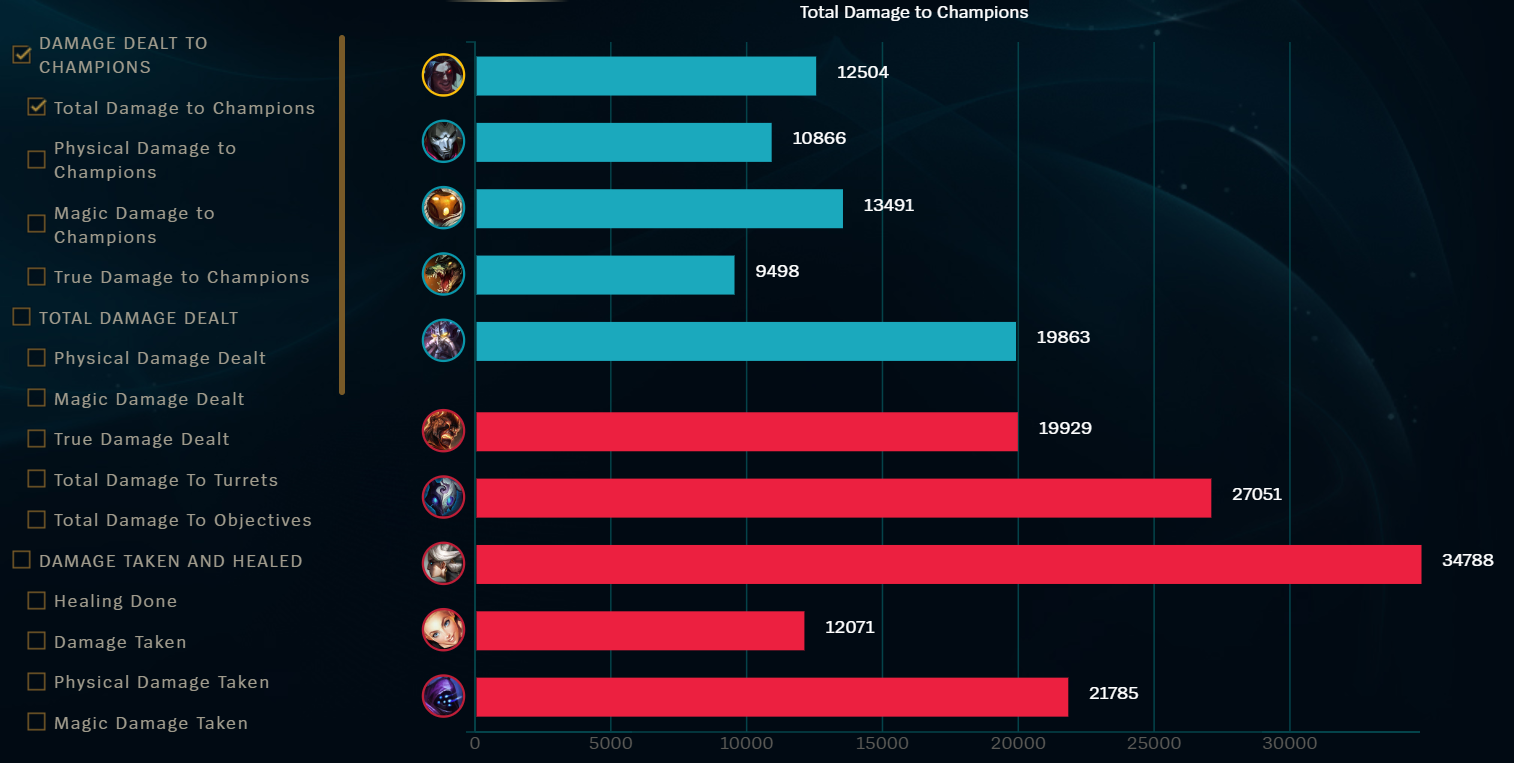
\includegraphics[width=\columnwidth, height=6cm]{source/images/lol_dmg_graph} }
	\label{fig:lol_stats}
	\caption[League of Legends: Post-Game Statistics]{There are two possibilities to see the in-game stats. Variation of (a) lists all values in tables. In variation (b) the numerical values are illustrated in graphs and can be selected in the menu. Around half of the available values are illustrated in this figure. Source: Adapted from \cite{LeagueClient} }
\end{figure}


\chapter{Experiment results}
\begin{table}[H]
	\caption[Average results of agents with respect to sub-tasks] {Average results of agents with respect to sub-tasks}
	\centering
	\scalebox{0.7}{\begin{tabular}{l*{8}{c}} 
		\hline \\ 
		Algorithm&Pellets&Power Pellets&Fruits&Ghosts&Ghosts x2&Ghosts x3&Ghosts x4   \\  [2ex] 
		\hline \\
		A2C & 59 & 1.4& 0& 0.7 & 0.1 & 0 & 0 \\ [2ex]
		Apex &  424 & 11.2 & 0.9 & 7.1 & 1.8 & 0.6 & 0\\ [2ex]
		DQN &  298 & 8 & 0 & 4 & 0 & 0 & 0 \\ [2ex]
		ES  & 59.5 & 1 & 0.4 & 1 & 1 & 0.3 & 0\\ [2ex]
		GA &  23.6 & 0.6 & 0 & 0 & 0 & 0 & 0 \\ [2ex]
		Rainbow &  147 & 4 & 1 & 3 & 0 & 0 & 0\\  [2ex]
		\hline
	\end{tabular}}
	\label{tab:eva2}
\end{table} 

\begin{table}[H]
	\caption[Average results of agents in level one] {Average results of agents in level one}
	\centering
	\scalebox{0.7}{\begin{tabular}{l*{6}{c}} 
		\hline \\ 
		Algorithm&Lives&Rewards&\%-Pellets&\%-Fruits&\%-Ghosts   \\  [2ex] 
		\hline \\
		A2C & 0 & 767 & 35.78 & 1.67 & 4.38  \\ [2ex]
		APEX & 1.93 & 2110 & 100.00 & 35.00 & 10.63 \\ [2ex]
		DQN & 2 & 1900 &100.00 & 0.00 & 6.25  \\[2ex]
		ES & 0 & 1575 & 38.33 & 15.00 & 15.00 \\ [2ex]
		GA & 0 & 290 & 17.00 & 0.00 & 0.00  \\ [2ex]
		Rainbow &  0 & 2370 & 98.00 & 50.00 & 18.75\\ [2ex]
		\hline
	\end{tabular}}
	\label{tab:eva3}
\end{table} 

\begin{table}[H]
	\caption[Average results of agents with 5\% random action probability] {Average results of agents with 5\% random action probability}
	\centering
	\scalebox{0.7}{\begin{tabular}{l*{6}{c}} 
		\hline \\ 
		Algorithm&Lives&Rewards&\%-Pellets&\%-Fruits&\%-Ghosts   \\  [2ex] 
		\hline \\
		A2C & 0.00  & 863.33 & 35.78 & 10.00 & 5.63 \\ [2ex]
		APEX & 1.60 & 2169.67 & 99.76 & 53.33 & 9.79 \\ [2ex]
		DQN & 0.63 & 2585.00 & 95.17 & 48.33 & 20.00 \\ [2ex]
		ES & 0.00 & 1084.67 & 33.25 & 11.67 & 9.17 \\[2ex]
		GA & 0.00  & 547.67 & 27.94 & 0.00 & 2.08  \\ [2ex]
		Rainbow & 0.80  & 2458.67 & 96.67 & 28.33 & 17.29 \\  [2ex]
		\hline
	\end{tabular}}
	\label{tab:eva5}
\end{table} 

\begin{table}[H]
	\caption[Results of all agents in regards of equally weighted sub-tasks]{Results of all agents in regards of equally weighted sub-tasks}
	\centering
	\scalebox{0.7}{
	\begin{tabular}{l*{5}{c}} 
		\hline \\ 
		Algorithm& Total score & Pellet score & Fruit score & Ghost score   \\  [2ex] 
		\hline \\
		A2C & 0.14 & 0.12 &0.01& 0.01 \\ [2ex]
		Ape-X & 0.49& 0.33 &0.12& 0.04 \\ [2ex]
		DQN & 0.35& 0.33& 0.00& 0.02 \\ [2ex]
		ES & 0.23& 0.13 &0.05 &0.05   \\[2ex]
		GA & 0.06& 0.06 &0.00 &0.00    \\ [2ex]
		Rainbow & 0.56& 0.33& 0.17& 0.06  \\ [2ex]
		\hline
	\end{tabular}}
	\label{tab:eva7}
\end{table} 

\begin{table}[H]
	\caption[Results of all agents in regards of passive playstyle]{Results of all agents in regards of passive playstyle}
	\centering
	\scalebox{0.7}{
	\begin{tabular}{l*{5}{c}} 
		\hline \\ 
		Algorithm& Total score & Pellet score & Fruit score & Ghost score   \\  [2ex] 
		\hline \\
		A2C&0.23&	0.21&	0.00&	0.01 \\ [2ex]
		Ape-X&0.69&	0.60&	0.07&	0.02 \\ [2ex]
		DQN&0.61&	0.60&	0.00&	0.01 \\ [2ex]
		ES&0.29&	0.23&	0.03&	0.03 \\ [2ex]
		GA&0.10&	0.10&	0.00&	0.00 \\ [2ex]
		Rainbow&0.73&	0.59&	0.10&	0.04 \\ [2ex]
		\hline
	\end{tabular}}
	\label{tab:eva9}
\end{table} 

\begin{table}[H]
	\caption[Results of all agents in regards of aggressive playstyle]{Results of all agents in regards of aggressive playstyle}
	\centering
	\scalebox{0.7}{
	\begin{tabular}{l*{5}{c}} 
		\hline \\ 
		Algorithm& Total score & Pellet score & Fruit score & Ghost score   \\  [2ex] 
		\hline \\
		A2C&0.10&	0.07&	0.00&	0.03&	0.10 \\ [2ex]
		Ape-X&0.33&	0.20&	0.07&	0.06&	0.33 \\ [2ex]
		DQN&0.24&	0.20&	0.00&	0.04&	0.24 \\ [2ex]
		ES&0.20&	0.08&	0.03&	0.09&	0.20 \\ [2ex]
		GA&0.03&	0.03&	0.00&	0.00&	0.03 \\ [2ex]
		Rainbow&0.41&	0.20&	0.10&	0.11&	0.41 \\ [2ex]
		\hline
	\end{tabular}}
	\label{tab:eva10}
\end{table} 


\chapter{Action evaluation results} \label{app:aceva}
\begin{table}[H]
	\caption[Action-sequence counter for each agent] {Action-sequence counter for each agent}
	\centering
	\scalebox{0.7}{\begin{tabular}{l*{11}{c}} 
		\hline \\ 
		Algorithm&Noop&Up&Right&Left&Down&Upright&Upleft&Downright&Downleft&Change  \\  [2ex] 
		\hline \\
		A2C	& 34858	&22	&23	&9	&11	&5615	&2539	&25549	&4593	&19150 \\  [2ex] 
		Ape-X	&5166	&8212	&8296	&2706	&10565	&9598	&8201	&12858	&17048	&31014 \\ [2ex] 
		DQN	&4400	&21633	&800	&5600	&12499	&200	&3600	&30200	&13400	&25598 \\ [2ex] 
		ES&	0	&0	&0	&0	&0	&0	&31579	&1033	&37107	&13351 \\ [2ex] 
		GA	&0	&0	&0	&0	&0	&28568	&0	&22145	&0	&12449 \\ [2ex] 
		Rainbow	&6894	&8299	&9500	&4491	&6692	&10696	&2800	&18096	&17564	&32457 \\  [2ex]
		\hline
	\end{tabular}}
	\label{tab:eva8}
\end{table} 

\begin{figure}%
\centering
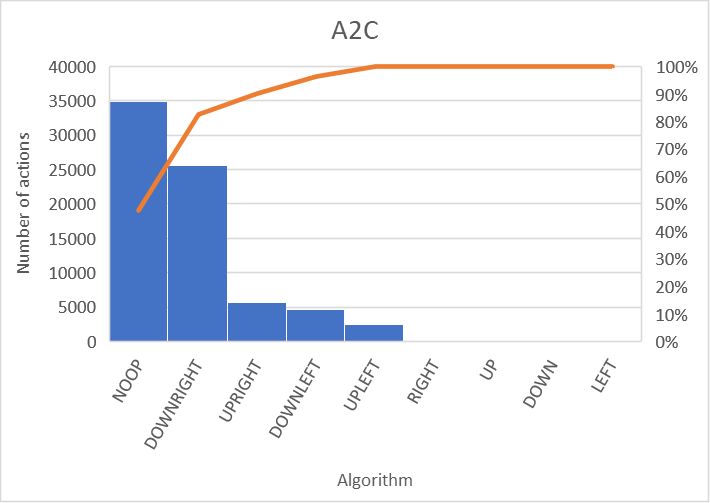
\includegraphics[scale=0.85]{source/images/eval/histo_a2c}%
\caption{Action-distribution of the A2C agent}%
\label{}%
\end{figure}

\begin{figure}%
\centering
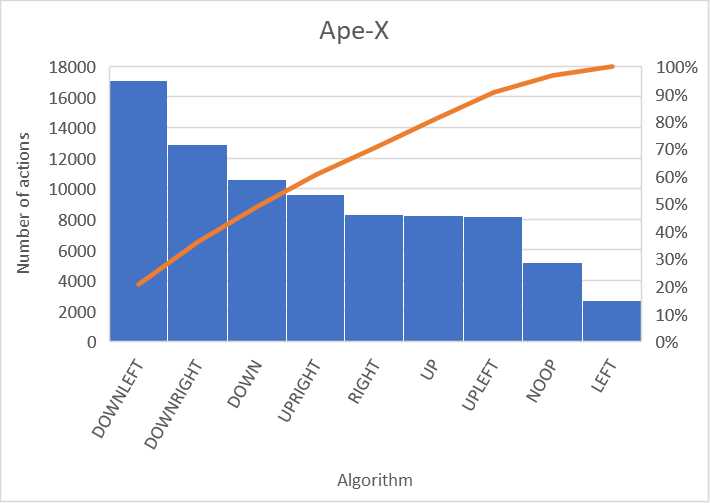
\includegraphics[scale=0.85]{source/images/eval/histo_apex}%
\caption{Action-distribution of the Ape-X agent}%
\label{}%
\end{figure}

\begin{figure}%
\centering
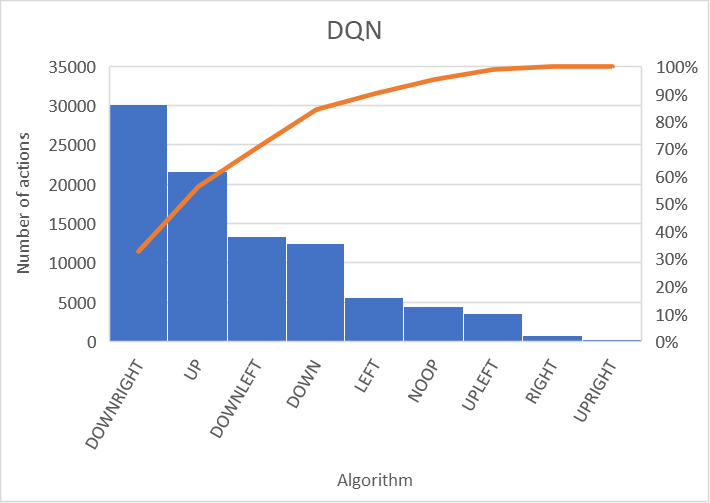
\includegraphics[scale=0.85]{source/images/eval/histo_dqn}%
\caption{Action-distribution of the DQN agent}%
\label{}%
\end{figure}

\begin{figure}%
\centering
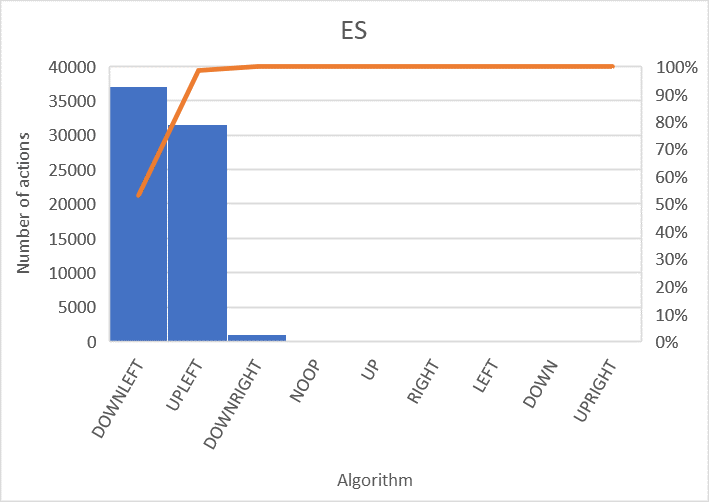
\includegraphics[scale=0.85]{source/images/eval/histo_es}%
\caption{Action-distribution of the ES agent}%
\label{}%
\end{figure}

\begin{figure}%
\centering
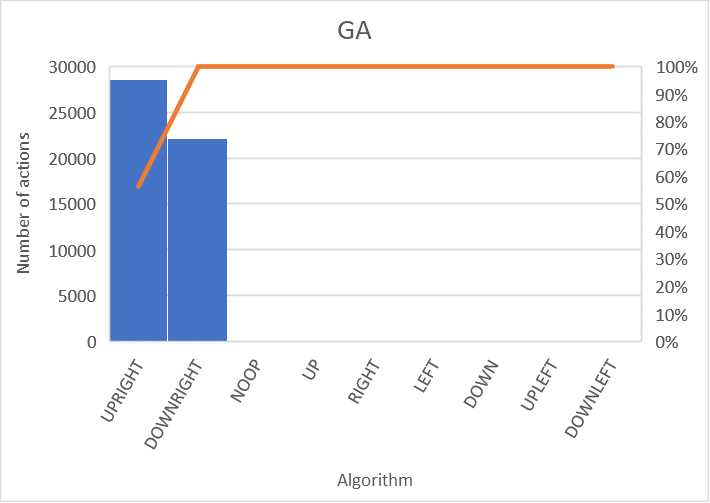
\includegraphics[scale=0.85]{source/images/eval/histo_ga}%
\caption{Action-distribution of the GA agent}%
\label{}%
\end{figure}

\begin{figure}%
\centering
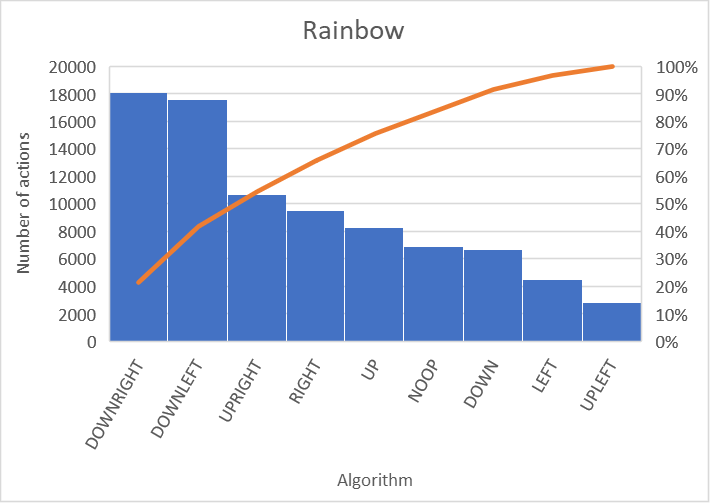
\includegraphics[scale=0.85]{source/images/eval/histo_rain}%
\caption{Action-distribution of the Rainbow agent}%
\label{}%
\end{figure}
